За работа с LaTeX има два основни начина - на локалната машина и в облачна услуга. Най-популярната облачна услуга е Overleaf, като тя дава множество възможности и е изключително лесна за усвояване, ако потребителят вече има опит с някоя от локалните инсталации на LaTeX системата. В настоящето изложение ще бъде представена интегрираната среда за създаване на документи Texmaker, в комбинация с MiKTeX, под операционна система Microsoft Windows.

\section{Инсталиране на MiKTeX}

MiKTeX е дистрибуция на TeX/LaTeX системата, работеща под операционна система Windows. Предоставя изчерпателен набор от инструменти и пакети за създаване и форматиране на документи, особено в академични и научни области. MiKTeX включва необходимите програми, шрифтове и макроси за ефективна работа с TeX/LaTeX на операционна система Windows. Той опростява процеса на инсталиране и гарантира, че потребителите ще имат достъп до различни пакети и ресурси за подготовка на документи.

Инсталирането на MiKTeX започва със сваляне на инсталационния файл от официалният сайт на продукта (Фиг. \ref{figure-0001}).

\begin{figure}
  \centering
  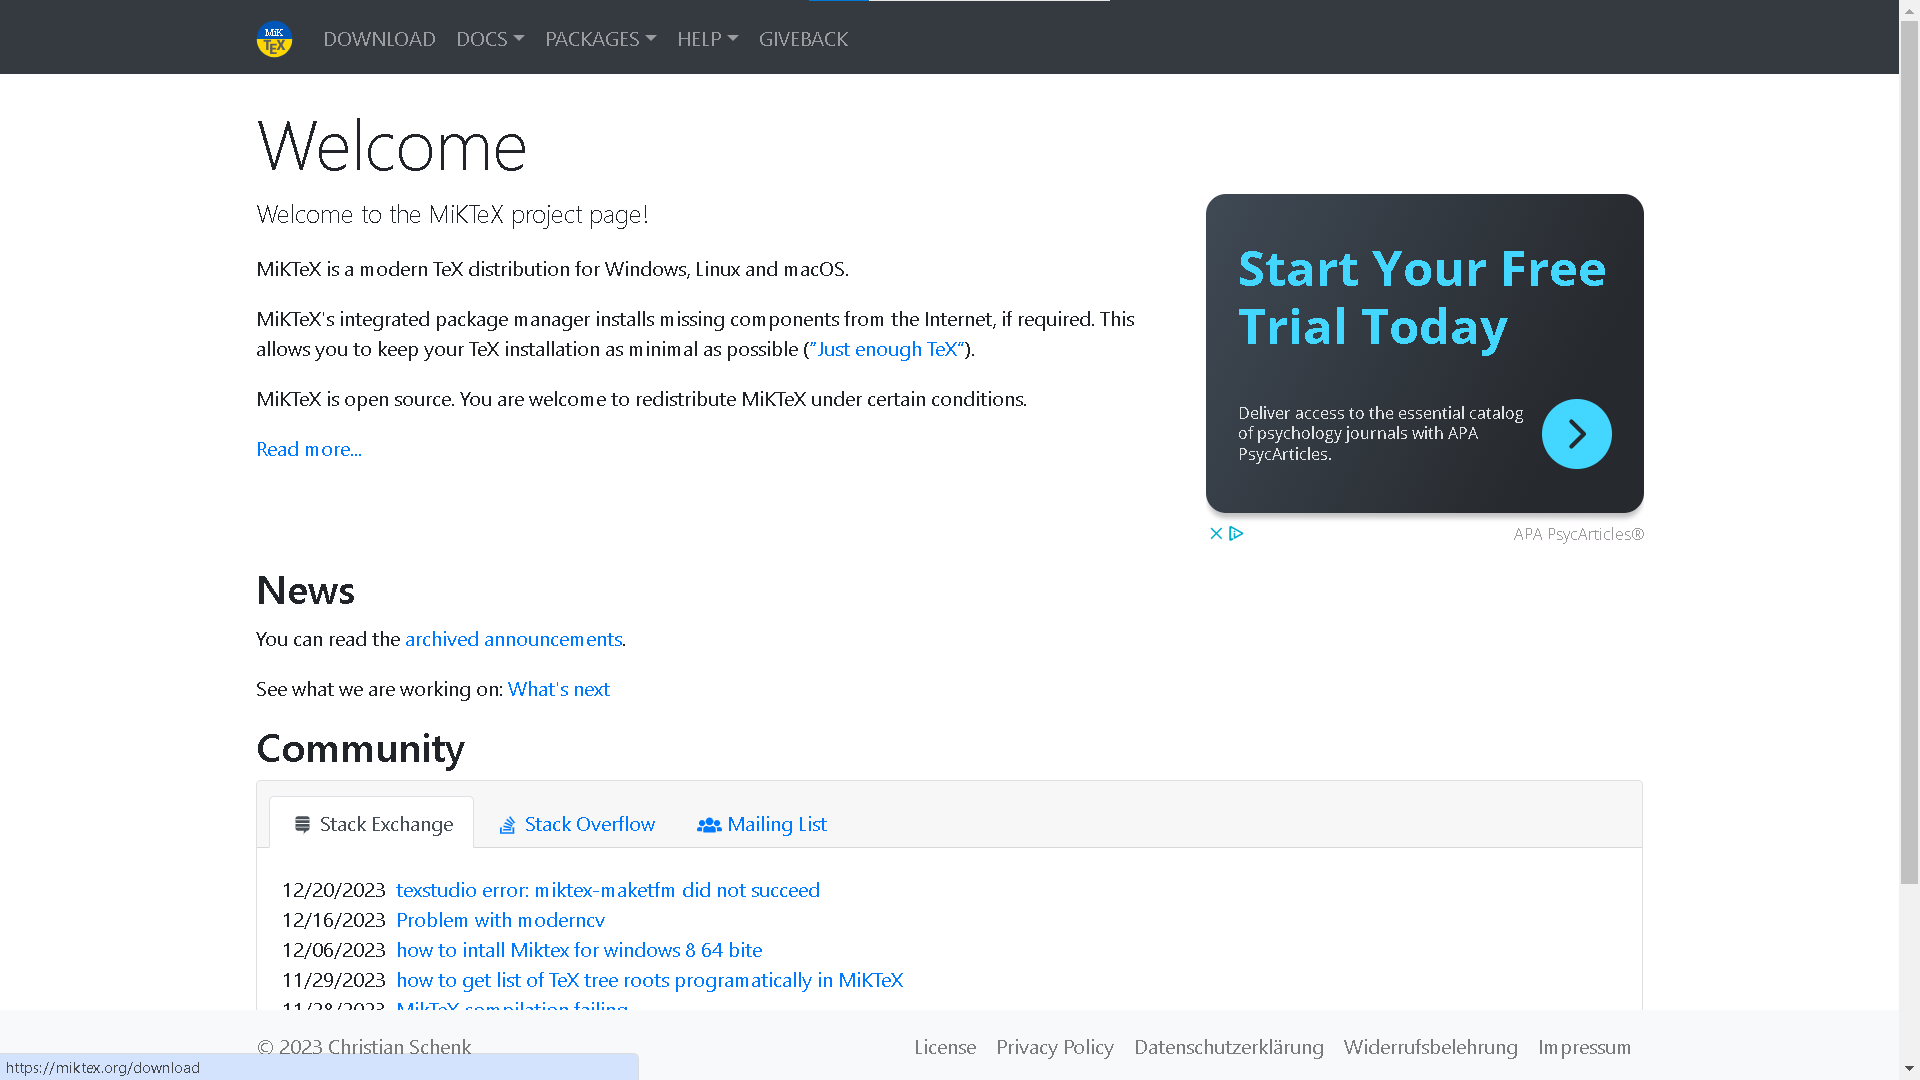
\includegraphics[width=1.0\linewidth,height=0.5\linewidth]{figure-0001.png}
  \caption{Начална уеб страница на MiKTeX}
\label{figure-0001}
\end{figure}

MiKTeX е достъпен за няколко различни операционни системи, но за нуждите на текущото изложение се използва версията на Windows (Фиг. \ref{figure-0002}).

\begin{figure}
  \centering
  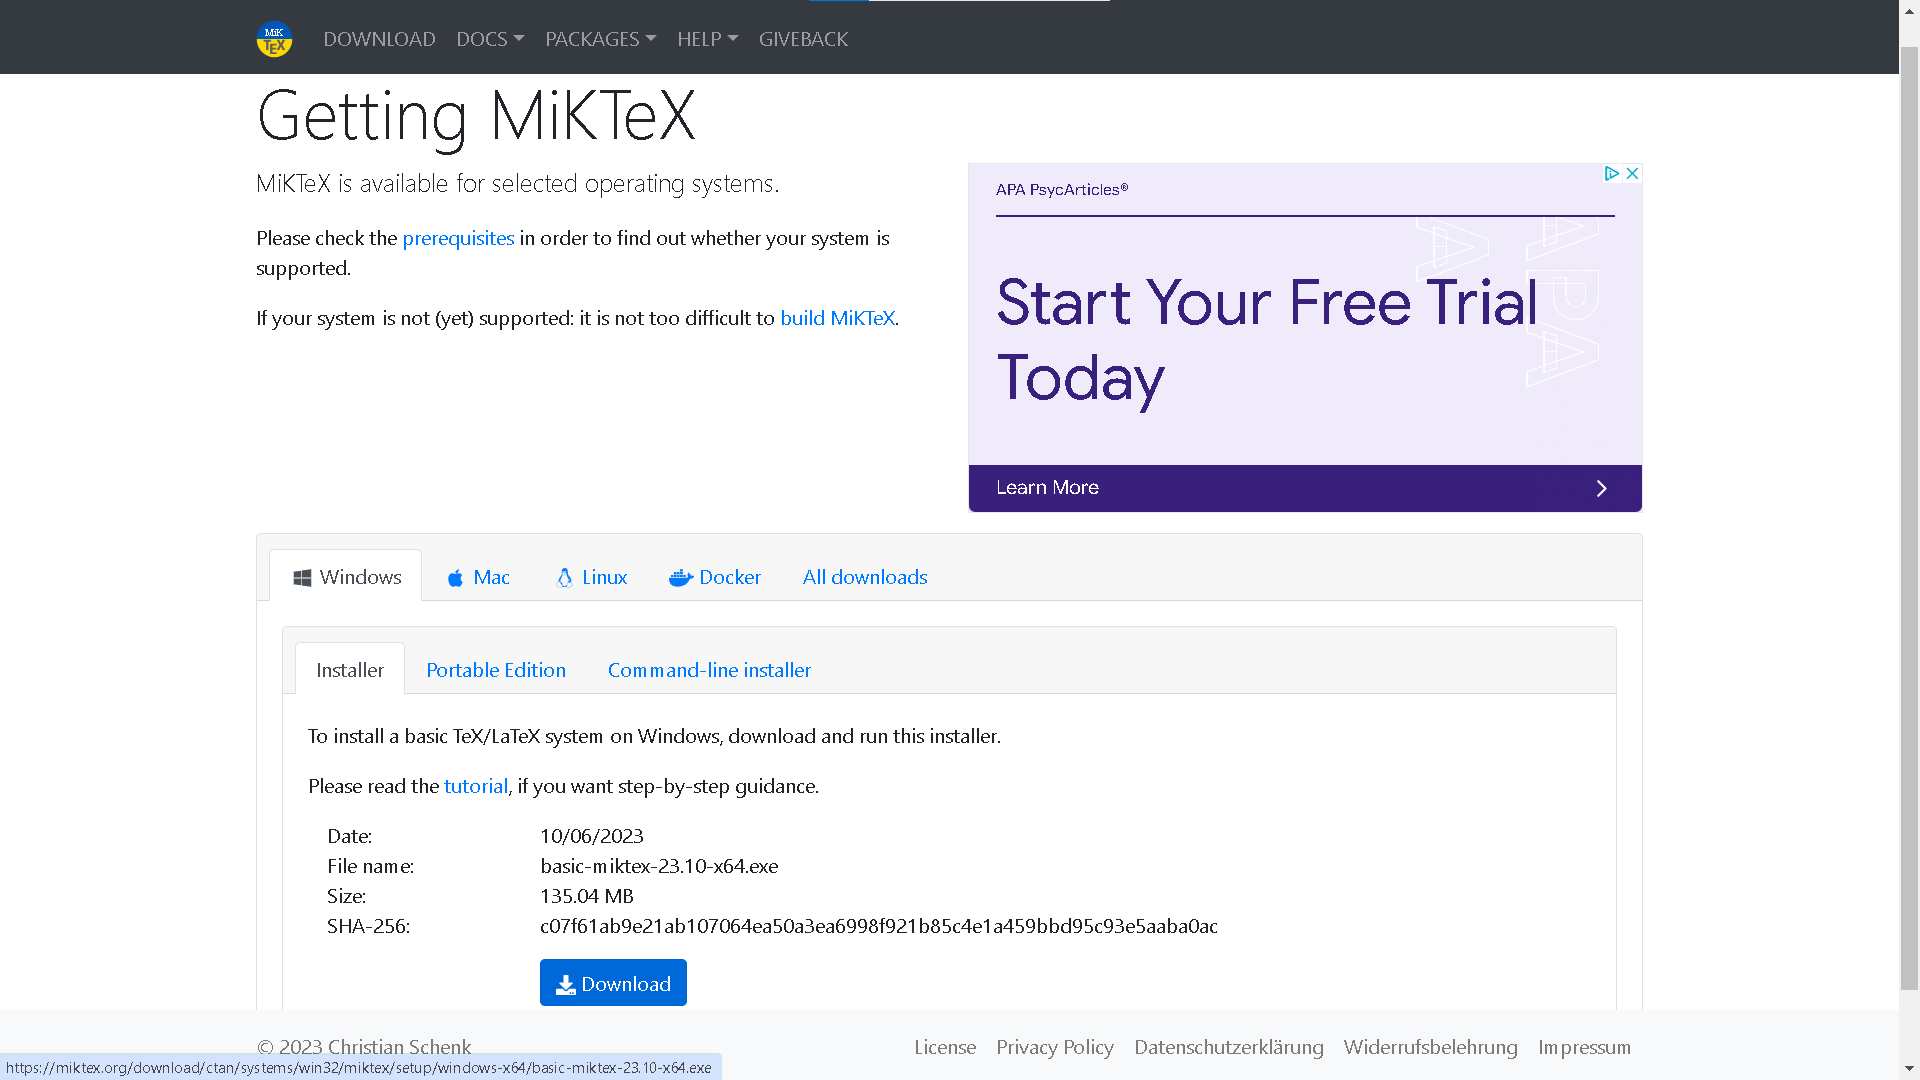
\includegraphics[width=1.0\linewidth,height=0.5\linewidth]{figure-0002.png}
  \caption{Избор на инсталационен файл за MiKTeX}
\label{figure-0002}
\end{figure}

Както всеки друг сериозен софтуерен продукт и MiKTeX е съпроводен с обши условия за ползване. Потребителят трябва да се съгласи с тях (Фиг. \ref{figure-0003}) веднага след като стартира изпълнимият файл на инсталатора.

\begin{figure}
  \centering
  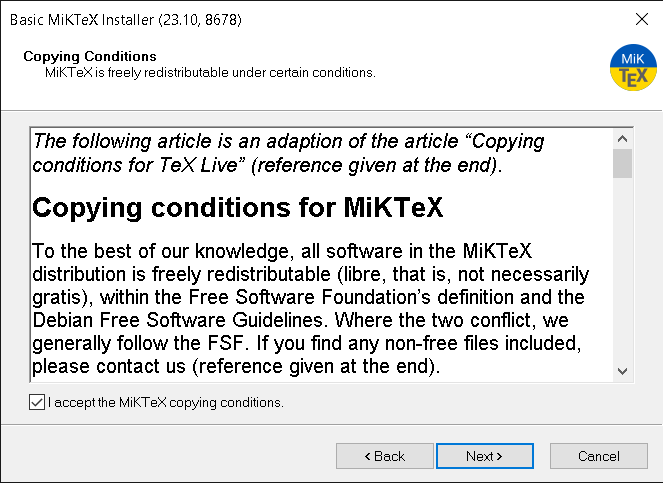
\includegraphics[width=1.0\linewidth,height=0.5\linewidth]{figure-0003.png}
  \caption{Диалогов прозорец за съгласие с условията за ползване на MiKTeX}
\label{figure-0003}
\end{figure}

Както при повечето съвременни операционни системи и в Windows се дава възможност за избор дали програмата да бъде инсталирана за конкретния потребители на системата (Фиг. \ref{figure-0004}) или за всички потребители.

\begin{figure}
  \centering
  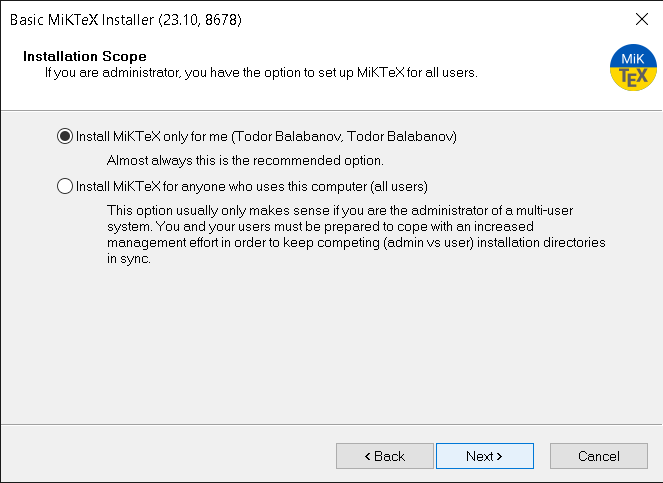
\includegraphics[width=1.0\linewidth,height=0.5\linewidth]{figure-0004.png}
  \caption{Избор на потребители с достъп до MiKTeX}
\label{figure-0004}
\end{figure}

За разлика от операционните системи, които под една или друга форма произлизат от операционната система Unix, в Windows потребителят сам трябва да посочи инсталационната директория (Фиг. \ref{figure-0005}) на софтуера, който той сам инсталира.

\begin{figure}
  \centering
  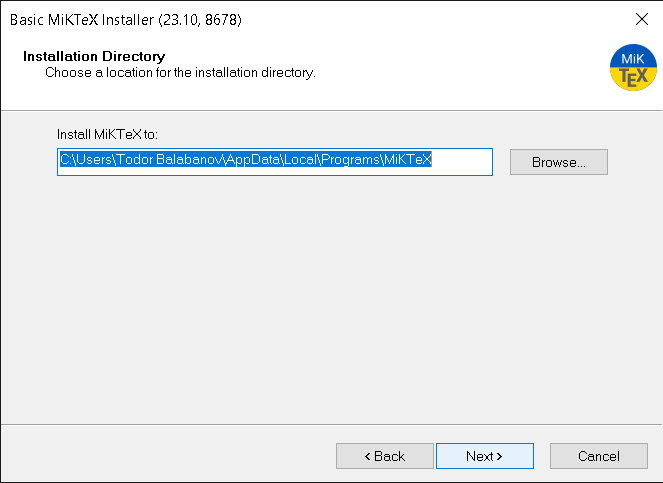
\includegraphics[width=1.0\linewidth,height=0.5\linewidth]{figure-0005.png}
  \caption{Инсталационна директория на MiKTeX}
\label{figure-0005}
\end{figure}

Тъй като LaTeX е система организирана на модулен принцип, към ядрото на системата могат да се инсталират допълнителни пакети. Не е нужно, а и би направило твърде тромава цялата система, ако всички налични пакети бъдат инсталирани предварително. Поради тези причини, допълнителните пакети се инсталират при първа поява за тяхната необходимост. При инсталирането на MiKTeX потребителят трябва да избере политиката за инсталиране на пакети. За да има контрол върху това, което бива инсталирано, то най-удачният избор е, при нужда от пакет, потребителят първо да бъде попитан (Фиг. \ref{figure-0006}).

\begin{figure}
  \centering
  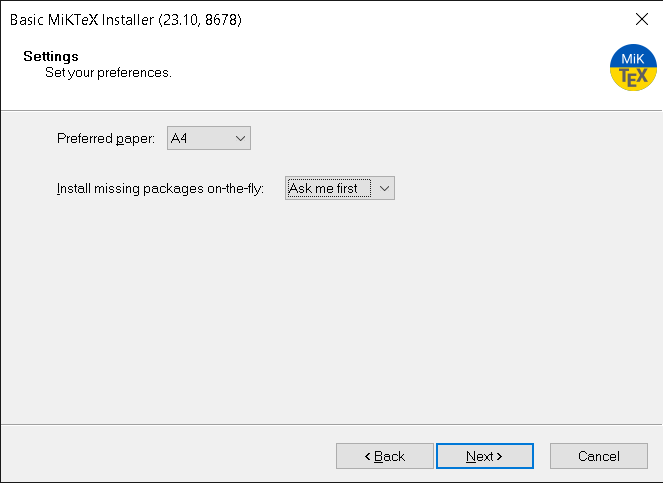
\includegraphics[width=1.0\linewidth,height=0.5\linewidth]{figure-0006.png}
  \caption{Избор на политика за инсталиране на пакети}
\label{figure-0006}
\end{figure}

След установяване на първоначалните параметри за изпълнение на инсталацията, процесът по инсталиране може да бъде стартиран (Фиг. \ref{figure-0007}).

\begin{figure}
  \centering
  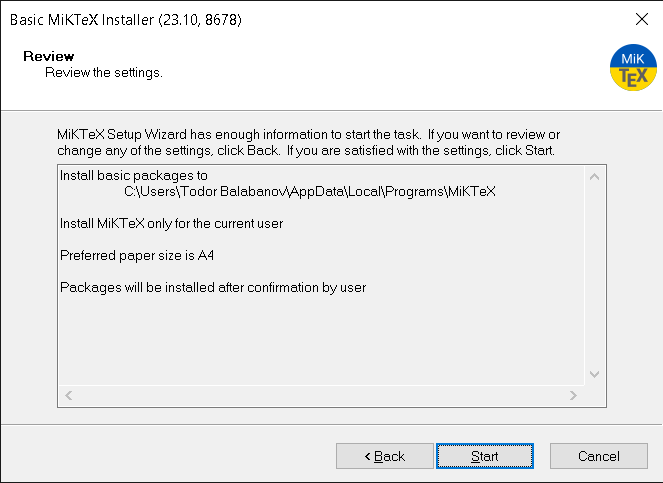
\includegraphics[width=1.0\linewidth,height=0.5\linewidth]{figure-0007.png}
  \caption{Стартиране на процеса по инсталация на MiKTeX}
\label{figure-0007}
\end{figure}

Чрез два прогрес бара, програмата за инсталиране на MiKTeX отразява напредъка в осъществяването на процеса (Фиг. \ref{figure-0008}).

\begin{figure}
  \centering
  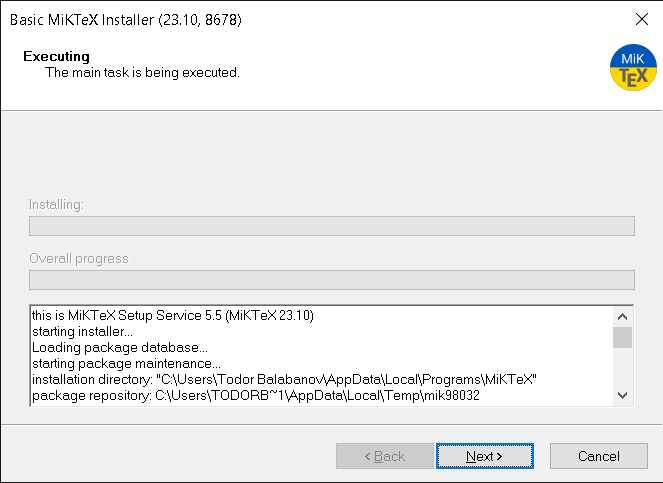
\includegraphics[width=1.0\linewidth,height=0.5\linewidth]{figure-0008.png}
  \caption{Прогрес на процедурата по инсталация}
\label{figure-0008}
\end{figure}

След инсталирането на основната част от продукта, потребителят има възможност да извърши проверка за наличие на нови версии (Фиг. \ref{figure-0009}).

\begin{figure}
  \centering
  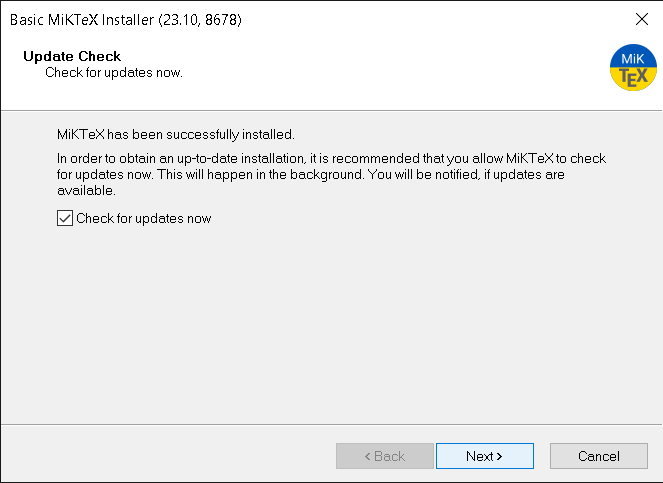
\includegraphics[width=1.0\linewidth,height=0.5\linewidth]{figure-0009.png}
  \caption{Избор за проверка на нови версии}
\label{figure-0009}
\end{figure}

Процедурата по инсталиране приключва със съобщение за начина по който е завършил процесът и с възможност за препращане към прозорец с допълнителна информация (Фиг. \ref{figure-0010}).

\begin{figure}
  \centering
  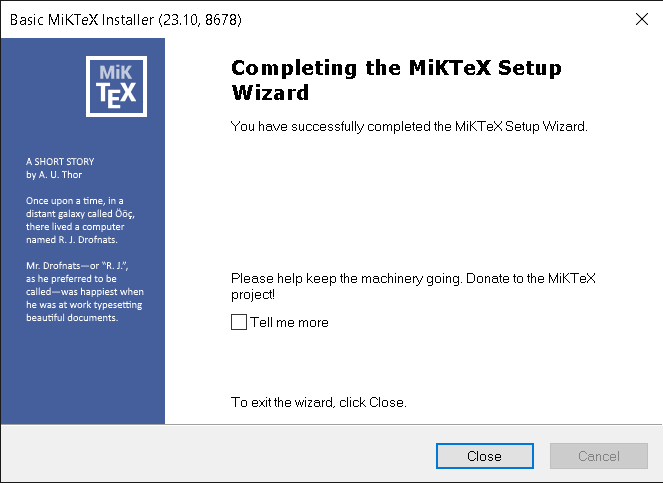
\includegraphics[width=1.0\linewidth,height=0.5\linewidth]{figure-0010.png}
  \caption{Диалогов прозорец с информация за извършеното инсталиране}
\label{figure-0010}
\end{figure}

MiKTeX осигурява основната функционалност за създаването на TeX документи, но за по-комфортна работа е разумно да се инсталира и специализиран текстов редактор.

\section{Инсталиране на Texmaker}

Texmaker е безплатен, многоплатформен LaTeX редактор, който предоставя интегрирана среда за разработка за работа със системата за набор на документи LaTeX. Той предлага удобен за потребителя интерфейс с функции като подчертаване на синтаксис, допълване на код, проверка на правописа и вграден PDF преглед за оформление на документи. Texmaker позволява на потребителите да създават и управляват LaTeX документи ефективно, като предлага инструменти за бърза навигация през големи документи, управление на множество файлове едновременно и компилиране на LaTeX код за генериране на PDF изход. Texmaker е предпочитан избор сред потребителите на LaTeX поради своята лекота на използване, гъвкавост и изчерпателен набор от функции за писане и редактиране на документи.

Както при MiKTeX, инсталирането на Texmaker започва със сваляне на инсталационния файл от официалният сайт на продукта (Фиг. \ref{figure-0011}).

\begin{figure}
  \centering
  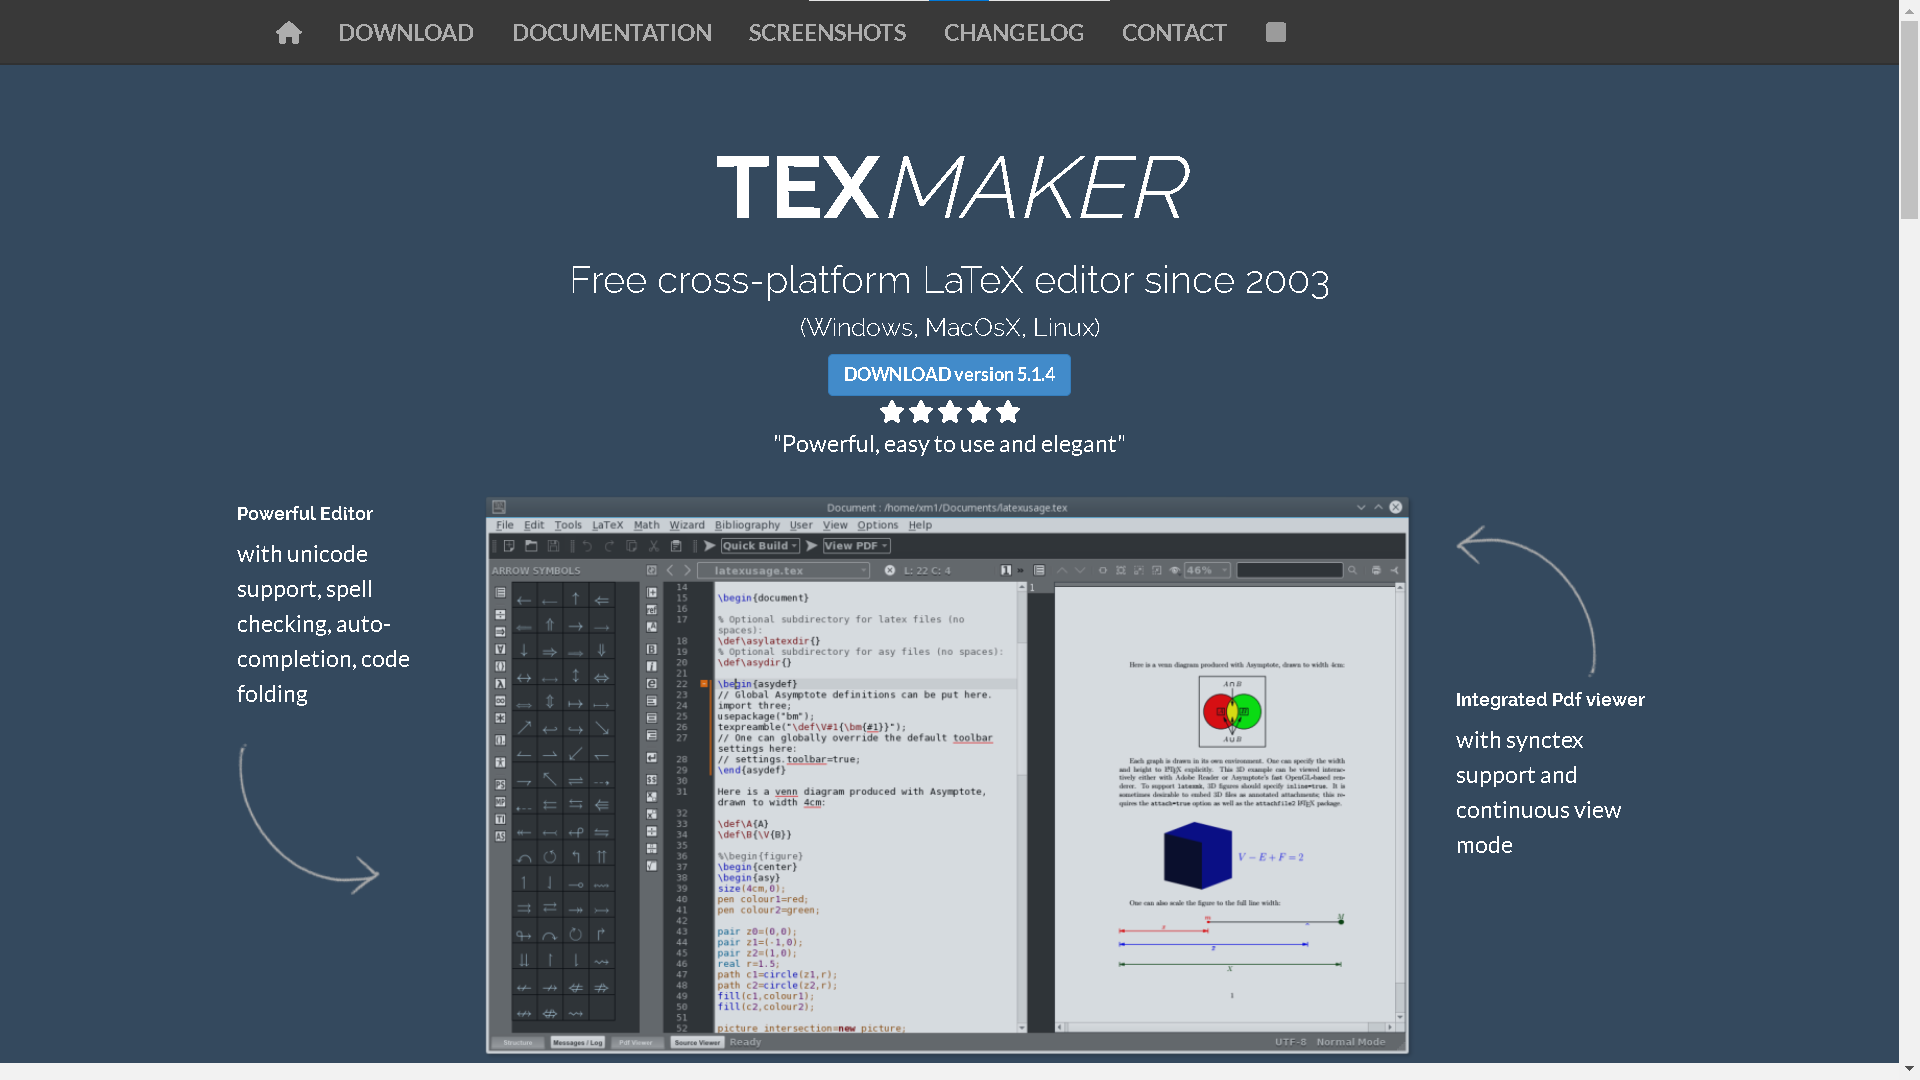
\includegraphics[width=1.0\linewidth,height=0.5\linewidth]{figure-0011.png}
  \caption{Начална уеб страница на Texmaker}
\label{figure-0011}
\end{figure}

Отново се избира тази версия за инсталиране, която е предназначена за използване под операционна система Windows (Фиг. \ref{figure-0012}).

\begin{figure}
  \centering
  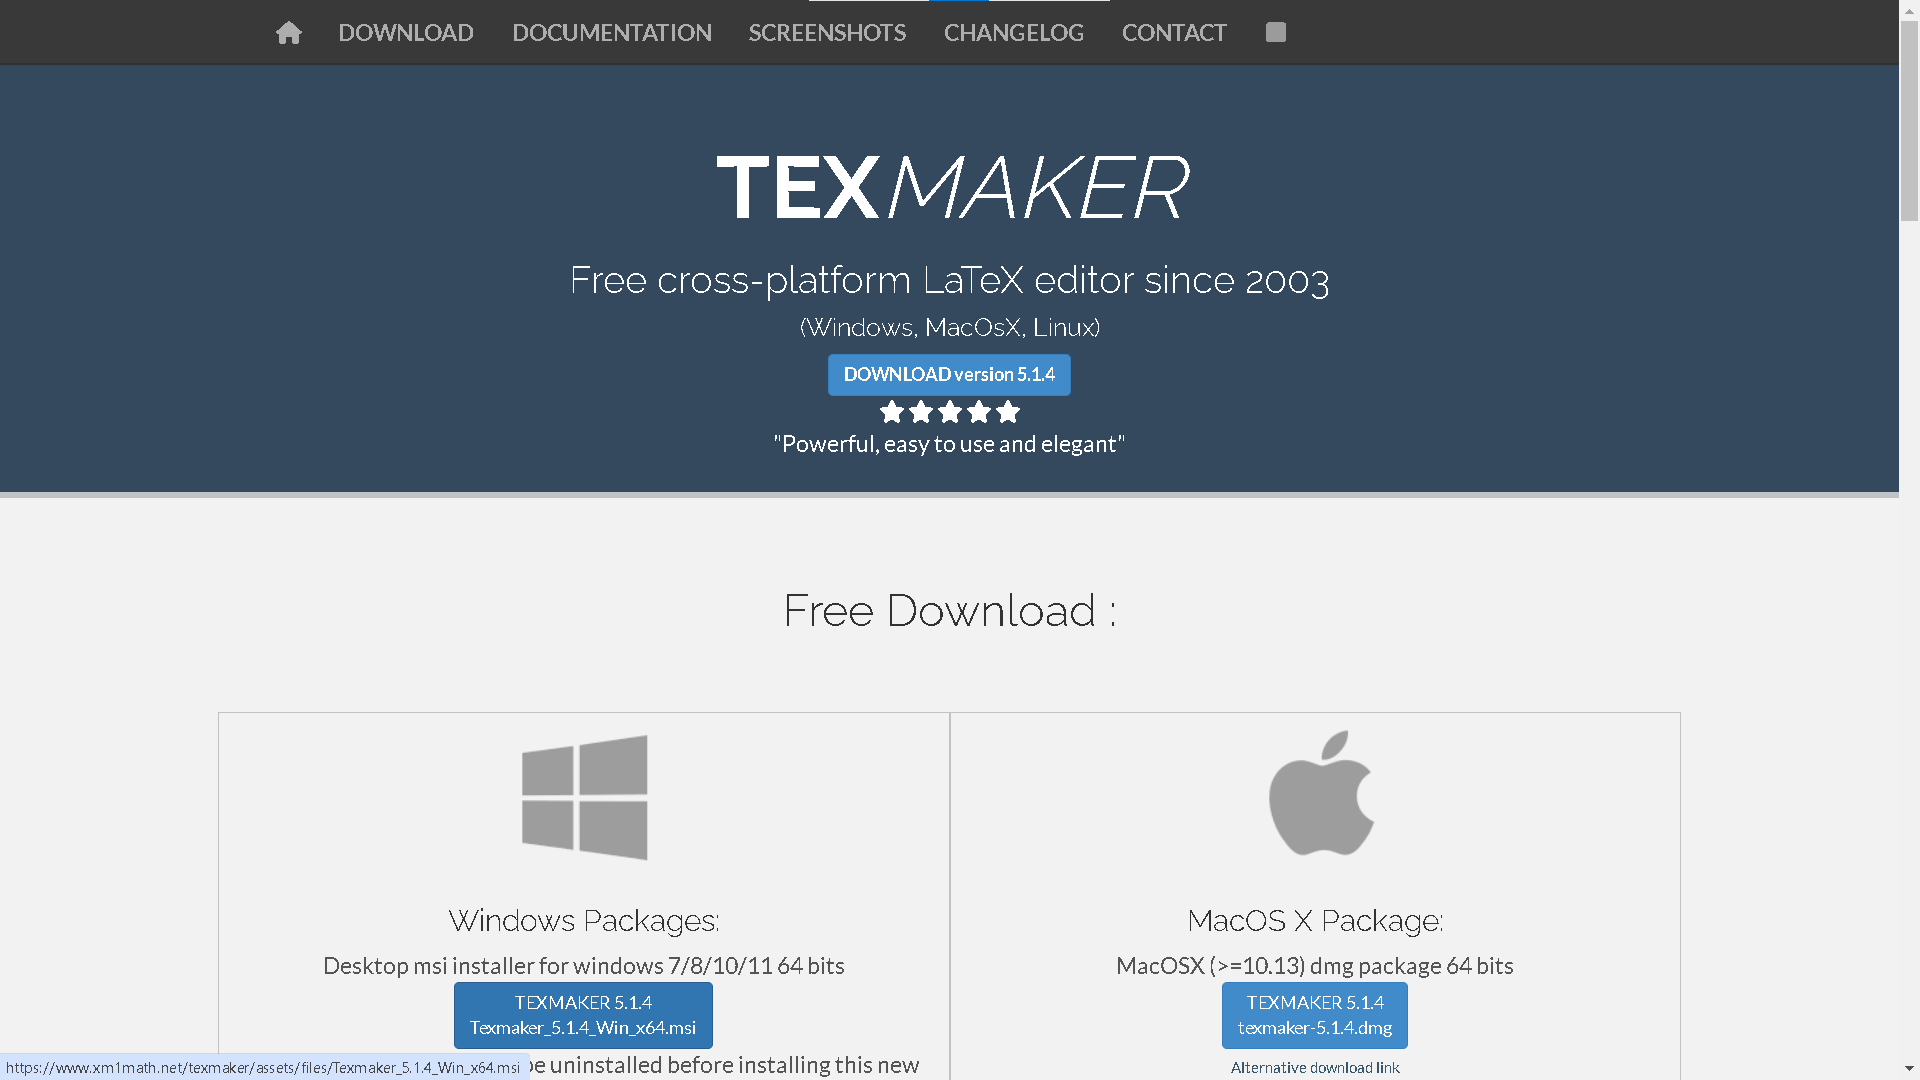
\includegraphics[width=1.0\linewidth,height=0.5\linewidth]{figure-0012.png}
  \caption{Избор на инсталационен файл за Texmaker}
\label{figure-0012}
\end{figure}

Потребителят бива информиран за юридическата рамка при която се съгласява да използва Texmaker, както и че за да бъде извършена инсталацията са необходими администраторски правомощия (Фиг. \ref{figure-0013}).

\begin{figure}
  \centering
  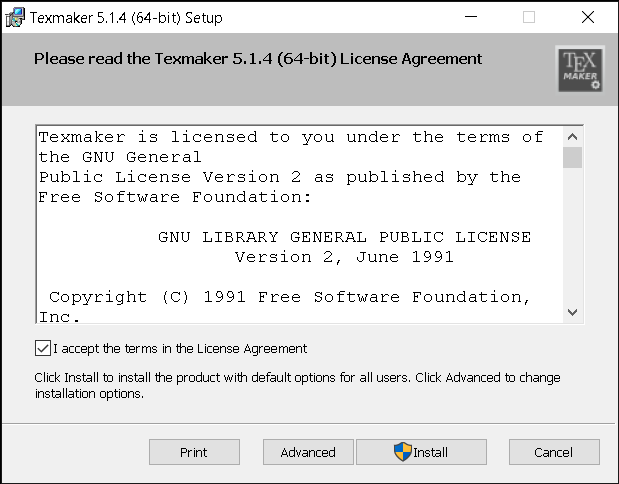
\includegraphics[width=1.0\linewidth,height=0.5\linewidth]{figure-0013.png}
  \caption{Диалогов прозорец за съгласие с условията за ползване на Texmaker}
\label{figure-0013}
\end{figure}

След приключване на процеса по инсталация, в диалогов прозорец се визуализира резултата и се дава възможност на потребителя да стартира програмата (Фиг. \ref{figure-0014}).

\begin{figure}
  \centering
  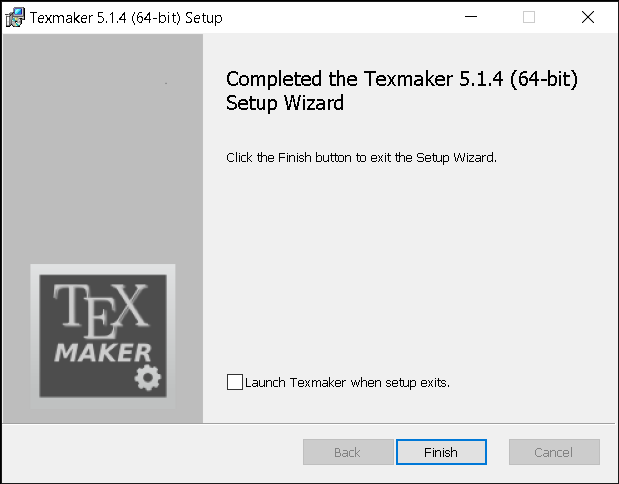
\includegraphics[width=1.0\linewidth,height=0.5\linewidth]{figure-0014.png}
  \caption{Диалогов прозорец с информация за извършеното инсталиране}
\label{figure-0014}
\end{figure}

Макар и успешно инсталирани, дали двата софтуера работят коректно най-добре може да се потвърди с изпълнението на минималистичен пример за LaTeX документ.

\section{Първоначален пример}



